\message{ !name(Worksheet 3 section 1.3.tex)}\documentclass[11pt]{exam}
\usepackage[margin=1in]{geometry}
\pagestyle{plain}
\usepackage{amsmath,amsfonts,amssymb,amsthm,enumerate}
\usepackage{multicol}
\usepackage[]{graphicx}
\usepackage{hyperref}
\usepackage{tikz}

\addtolength{\footskip}{2\baselineskip} % to lower the page numbers
\title{\vspace{-1.25in} Math 115 \\ Worksheet Section 1.3}
\date{}


% \theoremstyle{definition}
% \newtheorem{problem}{Problem}
\renewcommand{\questionlabel}{\textbf{Problem~\thequestion.}}
\printanswers

\begin{document}

\message{ !name(Worksheet 3 section 1.3.tex) !offset(99) }
A function has an inverse if and only if its graph
          intersects any horizontal line at most once. (See p. 27 of textbook.)
        \end{solution}
	
	\part Is $y=f(x) = 3x-5$ invertible?  If so, find the inverse.
        \begin{solution}
          Yes. We see \[
            y = 3x-5 \implies y-5 = 3x \implies x = \frac{y-5}{3}
          \]
        \end{solution}
	
	
	\part (1.3 \#19)
	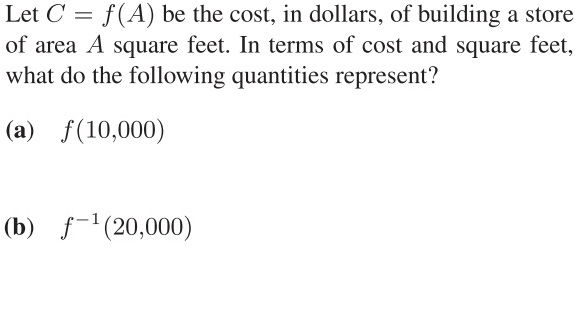
\includegraphics[width=3.5in]{no19.jpg}

\message{ !name(Worksheet 3 section 1.3.tex) !offset(171) }

  \end{document}
%%% Local Variables:
%%% mode: latex
%%% TeX-master: t
%%% End:
